\section{Yksikkötestityökaluja}

Androidin oma yksikkötestitapa on tehdä JUnit-testejä Androidin oman AndroidUnitTestCase-luokan aliluokkana. Nämä testit ajetaan emulaattorissa Dalvik-ympäristössä. Tässä tavassa on kaksi heikkoutta, jonka takia on olemassa myös kolmansien osapuolien yksikkötestityökaluja Android-ympäristöön. Ensinnäkin testien ajaminen emulaattorissa on hitaampaa kuin jos niitä voisi ajaa suoraan standardissa Javan virtuaalikoneessa JUnit-testeinä. Toiseksi muutkaan testauksen apuna käytettävät työkalut, kuten mock-kehykset, eivät välttämättä toimi ongelmitta Dalvik-ympäristössä. Tässä luvussa vertailen Android-sovelluksen yksikkötestausta AndroidUnitTestCasella ja suosituimmalla JVM-vaihtoehdolla: Robolectricillä.

Yksikkötesteissä kiinnostavaa on nimenomaan Androidin keskeisten komponenttien testauksesta, koska ohjelmassa mahdollisesti olevat muut kuin Androidin kirjastoluokista perivät luokat on helppo testata tavanomaisilla javan yksikkötestityökaluilla ilman erityisesti Androidille tarkoitettuja työkaluja.

Tavoitteista: helppokäyttöinen,nopea, toimii mock-kehysten kanssa, lue lisää lähteistä

\subsection{Robolectric}

Robolectric on yksikkötestaustyökalu, jonka tarkoitus on mahdollistaa android-koodin yksikkötestaus suoraan ohjelmointiympäristössä Javan virtuaalikoneessa ilman emulaattoria. Tarkoitus on mahdollistaa nopea TDD-sykli ja helpompi integrointi jatkuvan integroinnin palveluihin. Normaalisti Android-kirjaston luokat palauttavat kutsuttaessa IDE:stä ajoaikaisen poikkeuksen, mutta Robolectric korvaa nämä luokat varjototeutuksilla, jotka palauttavat poikkeuksen sijaan tyhjän oletusvastauksen (kuten null, 0 tai false) tai jos Robolectricissa on kyseistä metodia varten olemassa varjototeutus, se palauttaa toteutuksen määrittelemän oikeamman paluuarvon.

Robolectricin varjoluokkien käytön vaihtoehtona on jonkin mock-kehyksen käyttäminen androidin kirjaston korvaamiseen, mutta tämä on hyvin työläs ja verboosi tapa kirjoittaa testejä. Lisäksi tällöin testejä kirjoittaessa täytyy tuntea testattavan metodin toiminta hyvin tarkasti, jotta mock-toteutukset saadaan kirjoitettua. Robolectricin varjoluokat mahdollistavat enemmän musta laatikko -tyyppisen testauksen. \cite{robolectric}

\subsection{Aiempaa tutkimusta}

Sadeh et al. vertasivat Androidin aktiviteettien yksikkötestausta JUnitilla, AIT:lla (lyhenne/suomennos?) ja Robolectricilla. JUnitilla testattaessa ongelmaksi muodostui se, että ohjelmakoodia jouduttiin melko rajusti refaktoroimaan(suomennos?), jotta luokkien yksikkötestaus onnistui. Tämä tekee ohjelman ylläpidon vaikeaksi. JUnitin hyvä puoli oli erittäin nopea testien ajonopeus. Robolectricillä testien tekeminen taas oli lähes yhtä helppoa kuin AIT:lla. AIT:hen verrattuna Robolectricin vahvuudet oli virhepaikkojen paikantamisen helppous ja nopea ajonopeus. Robolectric-testit ajautuivat viisi kertaa nopeammin kuin AIT:lla ajetut testit, koska AIT ajaa testit emulaattorilla Dalvikilla, Robolectric taas suoraan Javalla. AIT:n suurin vahvuus oli testien kirjoittamisen helppous.\cite{sadehetal11}

Sadeh et al. eivät käyttäneet JUnit-testeissään mitään mock-työkalua, joten testeissä testiluokan riippuvuudet mockattiin tekemällä niistä staattisia sisäluokkia testiluokan sisään. Tämä on erittäin verboosi tapa ja vaikutti osaltaan siihen, miksi puhdas JUnit-testi näytti niin hankalalta. Androidin kirjastoluokat on pakko eristää testattavasta luokasta Javan virtuaalikoneella testattaessa, koska androidin kehitysympäristössä käytettävä paketti ei sisällä varsinaisesti luokkien sisältöä, vaan vain niiden luokkien julkiset rajapinnat, jolloin kehitystyökalut osaavat auttaa niiden käytössä, mutta varsinaista toteutusta ei ole.

Jeon \& Foster mainitsevat Robolectricin vahvuudeksi sen, että se pyörii Javan virtuaalikoneessa ja näin ohittaa hitaan vaihene testeistä, kun sovellus pitää kääntää emulaattorille tai laitteelle tetattavaksi. Robolectric ei heidän mielestään kuitenkaan sovellu kokonaisten sovellusten testaamiseen, koska sen varjoluokat eivät toteuta Androidin komponenteista kuin osan. Ylipäänsä Robolectric vertautuu Jeonin ja Fosterin mielestä paljolti robotiumiin. \cite{troyd}

Allevato \& Edwards käyttivät Robolectriciä opetuskäyttöön tarkoitetun RoboLIFT-työkalun kehitykseen. Robolectric auttoi heitä ohittamaan emulaattorin käytön ja nopeuttamaan opiskelijoiden testisykliä ja automaattista arviointialgoritmia. Tässä käytössä Robolectricin ongelma oli, että se ohittaa käyttöliittymän piirtämisen kokonaan ja muunmuassa näkymien onDraw-metodia ei kutsuta ollenkaan. Tämän seurauksena esimerksi näkymän leveys on aina 0 pikseliä, jolloin sellaiset testit, joilla haluttiin klikata näytöllä johonkin suhteelliseen kohtaan (vaikkapa keskelle) eivät toimineet oikein. \cite{robolift}

\subsection{Testiprojekti}

\begin{figure}[htb]
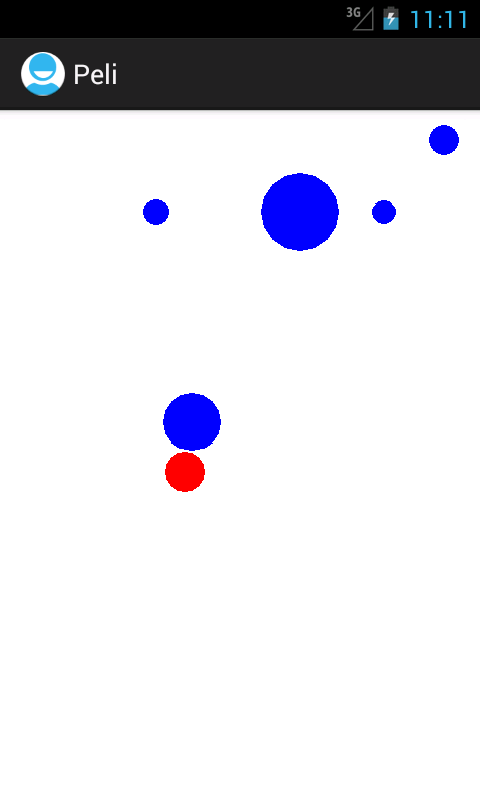
\includegraphics[width=60mm]{peli_screenshot.png}
\caption{Ruutukaappaus pelist} \label{peli_screenshot}
\end{figure}

Yksikkötestaustyökaluja testasin itse tehdyllä demoprojektilla. Kyseessä on yksinkertainen peli, jonka pelinäkymästä on ruutukaappaus kuvassa \ref{peli_screenshot}. Pelissä ohjataan kosketusnäytöllä painamalla punaista palloa ja pyritään väistämään ympäriinsä pomppivia sinisiä palloja. Kun peli päättyy, palataan takaisin päänäkymään, josta on ruutukaappaus kuvassa \ref{mainactivity}. Tästä näkymästä voi aloittaa uuden pelin ja lisäksi näkee, montako sekuntia edellinen peli kesti.

\begin{figure}[htb]
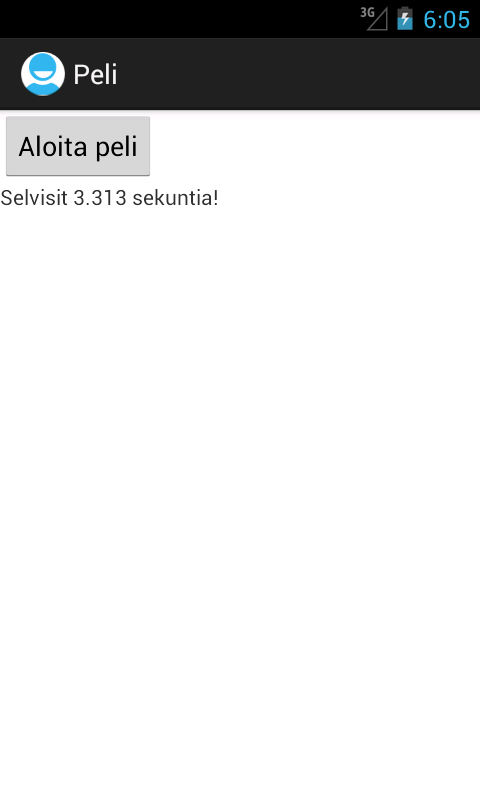
\includegraphics[width=60mm]{peli_mainactivity.png}
\caption{Ruutukaappaus pelist} \label{mainactivity}
\end{figure}

Peli koostuu kahdesta aktiviteetista, yksinkertaisemmasta MainActivity:sta sekä hieman monimutkaisemmasta GameActivity:sta, jonka yksikkötestaukseen keskityn. Itse peliä ohjaa GameView-luokka, joka on yhtä aikaa näkymä ja kontrolleri MVC-suunnittelumallin mukaisesti. Malleja ovat GameClock, joka kuvaa pelikelloa, sekä Circle, joka kuvaa yhtä ruudulla näkyvää ympyrää. GameActivity toteuttaa lisäksi OnGameEndListener-rajapinnan, jonka avulla GameView ilmoittaa pelin päättymisestä ja pistemäärästä. Pelin luokkakaavio on esitetty kuvassa \ref{game_classdiagram}.

\begin{figure}[htb]
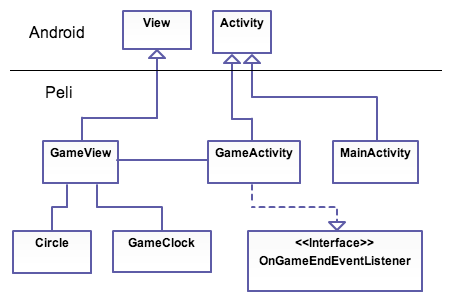
\includegraphics[width=110mm]{peli_luokkakaavio.png}
\caption{Pelin luokkakaavio} \label{game_classdiagram}
\end{figure}


\subsection{Robolectricin asentaminen}
\label{robolectric_install}

Robolectricin suositeltu asennustapa on Maven, joka on yleisesti käytössä oleva kääntämis- ja riippuvuuksienhallintatyökalu \cite{maven}. Koska testattava projekti ei ollut Maven-projekti, jouduin tekemään robolectric-testitkin ilman Mavenia. Ilman Mavenia asennus osoittautui haastavaksi: Eri kirjastopakettien riippuvuudet eivät tahtoneet mitenkään toimia yhteen. Lopulta asennus kuitenkin onnistui tekemällä Robolectricin TestRunnerista oma aliluokka. Listauksessa \ref{robolectric_runner} on muokattu Robolectricin aliluokka testejä varten lähteenä olleesta esimerkistä \cite{sample_runner}. Olennaista on, että yliluokalle syötetään konstruktoriparametrina RobolectricConfig-olio, jolle annetaan parametrina testattavan Android-sovelluksen AndroidManifest.xml sekä resurssi-hakemiston osoite.

\begin{lstlisting}[float,label=robolectric_runner,caption=CustomRobolectricTestRunner]
public class CustomRobolectricTestRunner 
       extends RobolectricTestRunner {
  public CustomRobolectricTestRunner(@SuppressWarnings("rawtypes")
                    Class testClass) throws InitializationError {
  	super(testClass, new RobolectricConfig(
                       new File("../Demo/AndroidManifest.xml"), 
                       new File("../Demo/res")));
  }
}
\end{lstlisting}

Robolectric-testejä varten luodaan oma tavallinen Java-projekti Eclipsessä, joka laitetaan viittaamaan Android-projektin koodiin. Testiprojektin build pathiin tarvitaan robolectricin jar-paketti, sekä androidin android.jar sekä maps.jar -paketit. Robolectricin paketin pitää olla riippuvuuslistassa ennen android-paketteja, jotta se toimii. Tämän jälkeen testejä voi ohjelmoida kuten tavallisia JUnit-testejä.

\subsection{Perusominaisuudet}
\label{basic_unittests}

Aktiviteetin elinkaarimetodien testaus on olennaisin osa android-sovellusten yksikkötestauksesta. Testeissä testataan koodia, joka löytyy liitteestä x.

\begin{lstlisting}[float,label=robolectric_activitytest,caption=Robolectric Activity test]
@RunWith(CustomRobolectricTestRunner.class)
public class GameActivityTest {

  private GameActivity activity;

  @Before
  public void setUp() {
    activity = new GameActivity();
    activity.onCreate(null);
  }

  @Test
  public void testCreatedActivityInitializesGameViewWithRunningState() throws Exception {
    GameView gameView = (GameView) activity.findViewById(R.id.gameview);
    assertThat(gameView.getState(), equalTo(GameState.RUNNING));
  }
  
  @Test
  public void testOnPauseStopsTheGame() {
  	activity.onPause();
  	GameView gameView = (GameView) activity.findViewById(R.id.gameview);
  	assertThat(gameView.getState(), equalTo(GameState.PAUSED));
  }
  
}
\end{lstlisting}

Listauksessa \ref{robolectric_activitytest} on yksinkertainen aktiviteettiyksikkötesti Robolectricillä toteutettuna. Robolectricin testit ovat yhteensopivia JUnitin version 4 kanssa, mikä mahdollistaa annotaatioiden käytön testeissä. @RunWith-annotaatiolla määritellään testien ajossa käytettävä testiajaja (runner), tässä tapauksessa käytetään luvussa \ref{robolectric_install} esiteltyä ajajaa. @Before-annotaatiolla ilmaistaan metodit, jotka on ajettava ennen testejä ja @Test-annotaatiolla ajettavat testit.

setUp()-metodissa alustetaan testattava aktiviteetti ja kutsutaan sen onCreate-metodia. Robolectric automaattisesti havaitsee Androidin metodien kutsun ja korvaa ne robolectricin toteutuksella, jotta ne toimivat testissä. Tämän takia aktiviteetti voidaan alustaa suoraan konstruktorilla ja kutsua sen onCreate()-metodia toisin kuin AndroidUnitTestissä, jossa aktiviteetti käynnistetään AndroidUnitTestCase-luokan apumetodien avulla.

Ensimmäisessä testissä testataan, että aktiviteetin onCreate()-metodista alustetaan GameView-olio Running-tilaan. Robolectricin toteutus findViewById()-metodista mahdollistaa View-olion löytämisen Android-sovelluksen resursseissa määritellyn tunnisteen perusteella. Tämän jälkeen varmistetaan, että GameViewin tila on todella vaihtunut Running-tilaan. 

Toinen testi on rakenteeltaan hyvin samanlainen: siinä testataan, että onPause()-elinkaarimetodin kutsuminen siirtää GameViewin pause-tilaan. Testimekaniikka on sinänsä täsmälleen samanlainen kuin ensimmäisessä testissä.

Nämä testit eivät vaadi mitenkään ottamaan huomioon, että testejä tehdään Robolectriciä, eikä oikeaa Androidia vastaan. Robolectric toimii taustalla automaattisesti ja mahdollistaa testien vaatimat Androidin kirjastokutsut.

\begin{lstlisting}[float,label=androidunit_activitytest,caption=ActivityUnitTestCase]
public class GameActivityTest extends ActivityUnitTestCase<GameActivity> {

  private GameActivity activity;

  public GameActivityTest() {
  	super(GameActivity.class);
  }

  public void setUp() throws Exception {
  	super.setUp();
  	startActivity(new Intent(getInstrumentation().getTargetContext(), 
  	              GameActivity.class), null, null);
    activity = (GameActivity)getActivity();
  }

  public void testCreatedActivityInitializesGameViewWithRunningState() {
    GameView gameView = (GameView) activity.findViewById(R.id.gameview);
    assertThat(gameView.getState(), equalTo(GameState.RUNNING));
  }
  
  public void testOnPauseStopsTheGame() {
  	activity.onPause();
  	GameView gameView = (GameView) activity.findViewById(R.id.gameview);
  	assertThat(gameView.getState(), equalTo(GameState.PAUSED));
  }
  
}
\end{lstlisting}

Listauksessa \ref{androidunit_activitytest} on toteutettu vastaavat testit kuin listauksessa \ref{robolectric_activitytest}. Itse testit ovat täysin identtisiä robolectric-testien välillä, erot ovat alustuksessa. Androidin aktiviteettiyksikkötestit perivät yliluokan ActivityUnitTestCase, jolle annetaan konstruktoriparametrina testattavan aktiviteetin luokka. Tämän jälkeen yliluokka instrumentoi luokan testausta varten.

setUp()-metodissa kutsutaan yliluokan setUp()-metodia ja käynnistetään testattava aktiviteetti yliluokan tarjoamalla startActivity()-metodilla. Tämän jälkeen viite testattavaan aktiviteettiin saadaan yliluokan getActivity()-metodilla.

Robolectricistä poiketen Androidin yksikkötestit ovat JUnit3-pohjaisia, joten annotaatioita ei käytetä, vaan metodien nimien perusteella päätellään setUp()-metodi sekä testimetodit siitä, että niiden nimi alkaa sanalla test. Koska setUp()-metodeita on vain yksi, on setUp()-metodin alussa kutsuttava yliluokan setUp()-metodia tai yliluokan suorittamat alustukset jäävät tekemättä.

\begin{lstlisting}[float,label=robolectric_shadow,caption=Robolectric Shadow objects]
@Test
public void testMainActivityIsCalledAfterLostGame() {
  GameView gameView = (GameView) activity.findViewById(R.id.gameview);
  gameView.setState(GameState.LOST);
  	
  ShadowActivity shadowActivity = shadowOf(activity);
  Intent startedIntent = shadowActivity.getNextStartedActivity();
  assertThat(startedIntent.getComponent().getClassName(), 
             equalTo(MainActivity.class.getName()));
  assertThat(startedIntent.getStringExtra(GameActivity.SCORE), 
             equalTo("0.0"));
}
\end{lstlisting}

Listauksessa \ref{robolectric_shadow} on hieman monimutkaisempi testitapaus samasta testiluokasta kuin listaus \ref{robolectric_activitytest}. Tässä testissä testataan että pelin loppua. Jos aktiviteetti toimii oikein, se rekisteröi GameView-oliolle observer-patternin (suomennos?) mukaisen tarkkailijan, jota kutsutaan, kun peli päättyy. Aktiviteetin pitäisi tämän jälkeen pyytää GameView-oliolta pistemäärä ja lähettää uusi aie, jolla käynnistetään MainActivity-aktiviteetti ja annetaan ylimääräisenä tietona saatu pistemäärä.

Androidin Activity-luokka ei tarjoa suoraa julkista metodia, jolla voitaisiin kysyä, minkä aikeen aktiviteetti on lähettänyt. Tällaisia tapauksia varten Robolectric tarjoaa varjo-olioita, jotka kopioivat oikean android-luokan tilan ja tarjoaa laajemman apin näiden olioiden tilaan. Tätä varten testissä tehdään varjo-olio testattavasta aktiviteetista ja varjo-oliolta voidaan kysyä getNextStartedActivity()-metodilla, mikä on seuraava käynnistettävä aktiviteetti. Tältä aikeelta voidaan sitten tarkistaa, että aktiviteetti lähetti aikeen MainActivity-aktiviteetin käynnistämiseksi ja ylimääräisenä tietona on pisteet, tässä tapauksessa 0.0, koska kello ei ole ollut testissä käytössä.

\begin{lstlisting}[float,label=android_intent,caption=ActivityUnitTestCase intents]
public void testMainActivityIsCalledAfterLostGame() {
  GameView gameView = (GameView) activity.findViewById(R.id.gameview);
  gameView.setState(GameState.LOST);
  	
  Intent startedIntent = getStartedActivityIntent();
  assertThat(startedIntent.getComponent().getClassName(), 
             equalTo(MainActivity.class.getName()));
  assertThat(startedIntent.getStringExtra(GameActivity.SCORE), 
             equalTo("0.0"));
}
\end{lstlisting}

Listauksessa \ref{android_intent} on toteutettu vastaava testi AndroidUnitTestCase:n avulla. Alustus tehdään testissä kuten Robolectric-testissäkin, mutta toiminnan varmistus on yksinkertaisempaa kuin Robolectricillä, koska AndroidUnitTestCase tarjoaa getStartedActivityIntent()-metodin, jolla saadaan aktiviteetin viimeisin lähettämä aie palautettua samalla tavalla kuin Robolectricin varjo-oliolta kysyttiin edellisessä listauksessa. Tämän jälkeen testin läpipääsyn varmistus tapahtuu täsmälleen samalla tavalla kuin Robolectric-testissä.

\subsection{Toiminta mock-kehysten kanssa}

Yksikkötestausta pyritään useimmiten tekemään niin, että testiluokka on eristetty riippuvuuksistaan. Apuvälineenä eristämisessä käytetään usein mock-kehyksiä. Näissä testeissä mock-kehyksenä käytetään Mockitoa, koska se toimii myös Androidissa sellaisenaan \cite{mockito}.

Luvussa \ref{basic_unittests} esitetyt yksikkötestit ovat riippuvaisia GameView-luokan toteutuksesta. Assertit voivat mennä väärin, jos GameView-luokan setState()-metodi ei muutakaan onnistuneesti tilaa. Tällöin kyse on kuitenkin GameView-luokan, eikä GameActivity-luokan toiminnasta. GameActivityn osalta testissä ollaan oikeastaan vain kiinnostuneita siitä, että aktiviteetin käynnistyessä pelin tilaa yritetään muuttaa RUNNING-tilaan.

\begin{lstlisting}[float,label=mock_subclass, caption=Mock Subclass]
private class MockGameActivity extends GameActivity {
	
	private GameView gameView;

  public MockGameActivity(GameView gameView) {
	  this.gameView = gameView;
  }

  @Override
  public View findViewById(int id) {
	  return gameView;
  }
}
\end{lstlisting}

Aktiviteetti on testissä eristettävä GameView:stä niin, että oikean näkymän sijaan se saa käyttöönsä mock-version näkymästä. Aktiviteetti käyttää findViewById()-metodia näkymän lataamiseen, koska se on alustettu layout-tiedostossa. Jotta tähän metodikutsuun pääsee väliin, täytyi aktiviteetille tehdä testiä varten aliluokka MockGameActivity, joka on esitetty listauksessa \ref{mock_subclass}. Aliluokka toteuttaa findViewById()-metodista version, joka palauttaa aina sille parametrina annetun näkymän, joka voi olla esimerkiksi mock-näkymä.

Tämän voisi robolectricillä tehdä vaihtoehtoisesti siten, että toteuttaa oman Shadow-luokan Activity-luokasta, joka on kaikkien aktiviteettien yliluokka. Toteutuksen voi tehdä siten, että käyttää Robolectricin oletustoteutusta kaikkeen muuhun paitsi findViewById()-metodin toteutukseen \cite{robolectric}. Mock-näkymän injektointia varten tälle voisi tehdä myös oman set-metodin, jolla mock-näkymä sijoitettaisiin palautettavaksi. Yllä esitetty testattavan luokan aliluokka on kuitenkin helpompi tapa toteuttaa sama asia, koska robolectricille ei tarvitse erikseen sanoa, että käyttää shadow-luokkana omaa toteutusta. Lisäksi on helpompi vaihdella, käytetäänkö testeissä omaa aliluokkaa, vai varsinaista testattavaa luokkaa. (tarkista vielä, että kuvattu tapa toimii käytännössäkin..)

\begin{lstlisting}[float,label=mock_test_robolectric, caption=Mock-testi robolectrcicillä]
@Test
public void testCreatedActivityInitializesGameWithRunningStateWithMock() throws Exception {
	GameView gameView = mock(GameView.class);
	activity = new MockGameActivity(gameView);
	activity.onCreate(null);
	verify(gameView).setState(GameState.RUNNING);
}
\end{lstlisting}

Listauksessa \ref{mock_test_robolectric} on esitetty edellisen listauksen aliluokkaa käyttävä robolectric-testi. Ensimmäisellä rivillä luodaan Mockiton mock-olio GameView-luokasta. Toisella rivillä luodaan testattavan aktiviteetin aliluokka, jolle syötetään mock-näkymä konstruktoriparametrina. Sitten kutsutaan onCreate-metodia, kuten listauksen \ref{robolectric_activitytest} vastaavassa testissä. Assertin sijaan testin läpäisy testataan Mockiton verify-metodilla, joka varmistaa, että parametrina annettua mock-olion annettua metodia kutsuttiin annetulla parametrillä.

\begin{lstlisting}[float,label=mock_test_android, caption=Mock-testi androidunittestillä]
@Test
public void testCreatedActivityInitializesGameWithRunningStateWithMock() throws Exception {
	GameView gameView = mock(GameView.class);
	MockGameActivity.setView(gameView);
	startActivity(new Intent(getInstrumentation().getTargetContext(), MockGameActivity.class), null, null);
	verify(gameView).setState(GameState.RUNNING);
}
\end{lstlisting}

AndroidUnitTestin avulla tehty vastaava testi listauksessa \ref{mock_test_android} on mock-näkymän luomisen ja testin läpäisyn varmistamisen kannalta täsmälleen samanlainen kuin robolectric-testi. Testissä käytetään apuna vastaavaa aliluokkaa kuin Robolectric-testissäkin ja aktiviteetin käynnistys tapahtuu samoin kuin listauksen \ref{androidunit_activitytest} testissä.

\subsection{TDD-syklin nopeus}

Robolectricin vahvuudeksi mainitaan toistuvasti sen testien ajonopeus. Testien ajonopeudella on merkitystä kahdesta syystä: ensinnäkin laajojen projektien tapauksessa testitapauksia voi olla hyvin paljon ja kaikkien testien ajo esimerksi ci-palvelimella (onko relevanttia mobiilissa, oisko parempia esimerkkejä?) voi kestää hyvin pitkään, mikä saattaa hidastaa koodin jakamista tai koodausprosessia, kun muutosten varmistus kestää pitkään.

Toinen, ehkä olennaisempi, tekijä on se, että yksikkötestausta tehdään nykyään usein Test Driven Development -prosessin mukaisesti siten, että ensin tehdään testi, joka testaa vielä olematonta koodia ja tämän jälkeen koodia muutetaan niin, että testi saadaan menemään läpi. Tällöin testejä ajetaan jatkuvasti ja ohjelmointiprosessi pysähtyy aina, kun odotetaan testien ajautumista ennen kuin päästään jatkamaan TDD-sykliä seuraavaan vaiheeseen. (Lähde TDD:lle, jne) Jos testien, edes yksittäisen testiluokan, ajaminen on kovin hidasta, tämä tekee TDD-tyylisestä ohjelmistokehityksestä liian hidasta, jotta se olisi käytännöllistä.

\begin{table}[h]
\centering
\begin{tabular}{ l l l l }
   & Keskiarvo (s) & Max (s) & Min (s) \\
  Robolectric & 1,59 & 1,61 & 1,577 \\
  AndroidUnitTest & 44,10 & 44,271 & 43,868 \\
\end{tabular}
\caption{Testikestot}
\label{unittest_timing}
\end{table}

Testasin ensin isomman testisetin ajonopeutta. Kopioin aiemmin luvussa esitellyn testiluokan mock-testin kanssa 32 erilliseksi testiluokaksi niin, että testimetodeita kertyi yhteensä 128. Ajoin kaikki testit yhtenä sarjana ja annoin Eclipsen ottaa aikaa testien suorituksesta. Tähän aikaan ei sisälly sitä aikaa, joka kuluu JUnitin käynnistymiseen. (Tämä aika on pitempi AUT:lle, mittaa). Toistin testit viisi kertaa ja testikestojen keskiarvo, maksimi ja minimi on esitetty taulukossa \ref{unittest_timing}. Testit ajoin Macbook Pro:lla OS X versiolla 10.7.5, joka oli varustettu 2.7Ghz Intel core i7 -tuplaydinprosessorilla ja 8 gigatavun muistilla.

Robolectricin testit kestivät keskimäärin 1,59 sekuntia, AndroidUnitTestilla 44,10 sekuntia. Testien ajaminen emulaattorissa oli siis noin 27 kertaa hitaampaa kuin Robolectricilla JVM:llä. Koska testattava sovellus ja itse testit ovat hyvin yksinkertaisia, on aikaero todennäköisesti vielä suurempi reaalimaailman tapauksessa. Robolectricin lupaus nopeammista yksikkötesteistä vaikuttaa siis toteutuvan.

Testisarjan lisäksi tutkin yksittäisten testien kestoja. Erityisen kauan emulaattorissa ajetuista testeistä kesti ensimmäisen testiluokan mock-testi. Sen ajo kesti jokaisella ajokerralla yli 12 sekuntia, eli yli 25\% koko testisarjan kestosta. Tämä johtunee siitä, että Mockito muokkaa ohjelman tavukoodia toimintaansa varten ja sen ensimmäinen alustus on hyvin hidas. Sama hitaus oli havaittavissa myös Robolectric-testeissä: ensimmäinen mock-testi kesti noin 0.3 sekuntia, mikä on noin 19\% koko Robolectric-testisarjasta. Suhteellinen hidastuminen on siis verrattavissa AndroidUnitTestillä ajettuihin testeihin.

Robolectricillä myös kaikkein ensimmäinen testi on hyvin hidas, noin 0.5 sekuntia. Robolectric toimii Mockiton tavoin tavukooditasolla ja instrumentoi jotain roskaa.. katso lähteistä.

Nämä seikat eivät kuitenkaan muuta kokonaiskuvaa siitä, että testien ajaminen on todella paljon nopeampaa Robolectricillä kuin AndroidUnitTestillä.

\begin{table}[h]
\centering
\begin{tabular}{ l l l }
   & Ensimmäisen testin alkuun (s) & Koko testisarjan loppuun \\
  Robolectric & 2.7 & 4.3 \\
  AndroidUnitTest & 36 & 80 \\
\end{tabular}
\caption{Testisarjan kesto alustus mukaanlukien}
\label{unittest_startup}
\end{table}

Toiseksi testasin, kuinka kauan kestää testikehyksen alustus siihen pisteeseen, että ensimmäinen testi lähtee ajautumaan koodimuutoksen jälkeen. Tämä tarkoittaa Android-tapauksessa sovelluksen asentamista emulaattoriin ja testikehyksen alustusta. Tulokset on esitetty taulukossa \ref{unittest_startup} Alustusajat olivat merkittäviä. Robolectricillä testikehyksen alustus kestää jopa kauemmin kuin koko 128 testin sarjan ajo ja AndroidUnitTestilläkin lähes yhtä kauan.

Aika ensimmäiseen testitulokseen on merkittävä ohjelmoidessa Test Driven Development (tdd) -filosofian mukaan. Tdd:ssä on kaksi merkittävää periaatetta: ohjelmakoodia saa kirjoittaa vain automaattisen testin korjaamiseksi ja duplikaattikoodin poistamiseksi. Näistä periaatteista seuraa tunnettu tdd-sykli: punainen, vihreä, refaktoroi. Ensin kirjoitetaan testi, joka ei mene läpi, koska testin toteuttavaa ohjelmakoodia ei ole vielä olemassa. Vaiheen nimi on punainen, koska useimmilla yksikkötestityökaluilla lopputuloksena näkyy punainen palkki, jos jokin testi ei mene läpi. Toinen vaihe on kirjoittaa juuri sen verran koodia, mitä tarvitaan testin läpäisemiseksi. Tässä vaiheessa ei välitetä miten rumaa koodi on. Vaiheen nimi on vihreä, koska useimmillaa yksikkötestityökaluilla lopputuloksena näkyy vihreä palkki, kun testit menevät läpi. Viimeisessä vaiheessa refaktoroidaan toisessa vaiheessa mahdollisesti syntynyt duplikaattikoodi. Refaktorointivaiheessa kirjoitetut testit auttavat varmistamaan, ettei refaktoroidessa hajoiteta vanhaa toiminnallisuutta. Jotta tällainen ohjelmointisykli on mahdollinen, yksi vaatimus on, että ohjelmointiympäristö tarjoaa nopean palautteen testeistä \cite{tdd}.

\subsection{Mitä jäi kokeilematta, puuttuvia featureja?}

Onko tällaisia? Entä muiden kuin aktiviteettien testaus robolectricilla. Mitä muuta on vielä käsittelemättä?

\subsection{Analyysi}

Ohjelmakoodin yksikkötestaus onnistui hyvin sekä androidin mukana tulevalla yksikkötestikehyksellä, että Robolectricillä. Itse testikoodi ei poikennut kovin merkittävästi toisistaan eri kehyksille kirjoitetulla koodilla ja testien kirjoitukseen ei tarvinnut kovin paljoa Android-specifiä osaamista. Robolectric-koodi oli jopa yksinkertaisempaa testattavien komponenttien alustuksen ostalta, koska konstruktoreja saattoi käyttää suoraan yliluokan tarjoamien alustusmetodien sijaan. Toisaalta joskus oli vaikea tietää, mitä metodeita eri luokkien valmiit shadow-toteutukset tarjoavat. Näissä tapauksissa AndroidUnitTestCasen yliluokkametodit olivat käytössä selkeämpiä. Toisaalta Robolectric tarjoaa mahdollisuuden kirjoittaa itse omia shadow-luokkia, joissa voi toteuttaa stubeja Androidin kirjastoluokkien toiminnalle, kuten itse haluaa.

Mock-kehyksen käyttö onnistui ongelmitta sekä Robolectricillä että AndroidUnitTestCasella. Mockito toimi suoraan yhdessä Robolectricin kanssa ja Android-emulaattorissa ajaminenkin vaati vain erillisen dalvik-käännöspaketin.

Suurin ero testityökalujen välillä oli testien suoritusnopeudella. Robolectric lupaa nopeita testejä ja toteuttaa lupauksensa; Robolectric-testit ajautuivat yli 20 kertaa nopeammin kuin emulaattorissa ajetut AndroidUnitTestit. Lisäksi AndroidUnitTestillä aika ensimmäiseen testitulokseen pienelläkin testiohjelmalla oli yli puoli minuuttia, joten tdd-filosofian mukainen ohjelmointi AndroidUnitTestCasea käyttäen on toivottoman hidasta.